% !TeX spellcheck = en_GB
%!TEX TS-program = xelatex
%!BIB TS-program = biber
\chapter{Thermal Analysis of Orientation Clustering}\label{chap:p5}
\section*{Statement of Contribution}
	This chapter includes a co-authored book chapter. The bibliographic details of the published chapter are:
\begin{itemize}
	\item Javanbakht, Z, Hall, W \& Öchsner, A (2019), “Effective Thermal Conductivity of Fibre Reinforced Composites Under Orientation Clustering”, In: Engineering design applications. Ed. by A Öchsner \& H Altenbach. Vol. 92. Advanced structured materials, 1869-8433, Cham, Switzerland: Springer, pp. 507–519.
\end{itemize}
	My contribution as the corresponding author to the paper involved: undertaking literature review, classifying the necessary theoretical backgrounds and models, developing the programming code, analysing and discussing the finite element results, drawing figures, preparing tables, writing and editing the manuscript according to my supervisors’ comments.

\Zia\\
\Wayne\\
\vfill
\newpage

% --------------------------------------------------------------------------------------------------
\paragraph{Title} Effective Thermal Conductivity of Fibre Reinforced Composites Under Orientation Clustering

\paragraph{Abstract} A parametric finite element analysis is carried out to investigate the sensitivity of the effective thermal conductivity of fibres to orientation clustering. Randomly-positioned fibres with von Mises orientation distributions were used in different considerations and volume fractions to generate the dispersion in a partitioned representative volume element. It was found that increasing the fibre volume fraction increases the thermal conductivity; this improvement is significant specially when a preferred orientation is detected with a cluster-free state. Further reinforcement of the composite is made possible by increasing the maximum principal value of the orientation tensor provided that the principal direction is set accordingly. Furthermore, clustering index seems to not be affected by volume fraction when an equal distribution is present in partitions.

\section{Introduction}
	Heat dissipation can be problematic in composites due to their low thermal conductivity and anisotropic nature~\autocite{Kalaprasad.2000}. There are several parameters which affect the thermal conductivity of fibre reinforced composites among which is the orientation of the fibres; it plays a key role in defining the internal structure of the composite~\autocite{Behzad.2007,Lee.2003}. Additionally, increasing the fibre volume fraction will initiate more interaction between the fibres specially in the concentrated regions. The effect of these two parameters couples together in non-dilute regions of moulding flows during injection moulding processes, i.e., volume fractions more than 1\% are more susceptible to fibre clustering~\autocite{Ranganathan.1990}. Further complication is introduced when the effect of interfacial thermal barrier resistance is considered. Namely, not merely the volume fraction but also the specific area of the inclusions is also influential~\autocite{Hasselman.1987}.
	
	Due to the aforementioned complications, among many others, evaluation of the thermal conductivity of various fibres of composites has been an attraction to researchers. Effective thermal conductivity of fibres in the transverse direction~\autocite{Liu.2012,Agrawal.2015,Qian.2016,Javanbakht.2018}, in-plane~\autocite{Villiere.2013,Behzad.2007}, and longitudinal direction~\autocite{Korab.2002,Yang.2005} has been investigated in the literature. Furthermore, three dimensional pseudo-random distribution of fibres is considered in~\autocite{Wang.2009,GomezMunoz.2008,Javanbakht.2016,Javanbakht.2016b,Kari.2007}. The anisotropic improvement of heat conduction is also investigated in several publications, see~\autocite{Tian.2012,Gori.2013}. Many of the analytical approaches tend to provide wide bounds, specially for high contrast heterogeneous media, rather than specific values~\autocite{Kanit.2003}. In addition, high contrast fibre reinforced composites show more sensitivity to clustering~\autocite{Kataoka.2000}. Therefore in this context, computational methods are favoured despite the fact that the results are more model-dependent. Such side effects should be smoothed by selecting appropriate representative volume elements (RVEs) and explicit consideration of fibre orientation.
	
	The orientation of fibres in a composite can be described statistically in a continuous manner using orientation distribution functions~\autocite{Nomura.1970}. The discretised alternative is using orientation tensors~\autocite{Scheidegger.1965,Advani.1987} which are evaluated for various regions of the medium to detect orientation clustering of fibres~\autocite{Lee.2003,Krause.2010,Sliseris.2016,Yang.2010}. Many high order orientation tensors are available in the literature~\autocite{DuChung.2002} but the second order orientation tensor is more frequent due to its simplicity. Although a second order orientation tensor is not deemed accurate enough to represent the micro-structure of a composite~\autocite{Muller.2016b}, it is adequate for calculations pertaining to thermal conductivity~\autocite{Ranganathan.1990}.
	
	In the current study, a mean field approach is adopted to correlate the effect of clustered fibres to the effective thermal conductivity. Computational analyses were carried out using the finite element method. Most of the numerical researches have used auxiliary programming languages, such as Mathematica~\autocite{GomezMunoz.2008}, to carry out the generation of pseudo-random fibre distribution. This requires a transfer of data between programs and some manual handling of the operations. Herein, an integrated Python script is used along with the MSC Marc commercial finite element package in a manner that the connection is automatically established and maintained. Furthermore, all supplementary calculations and post-processing tasks were handled by means of the same facility, for detailed information see \autocite{Javanbakht.2017}. A list of the used symbols in the current work is also provided for the convenience of the reader, see Table~\ref{table:symbols5}.
\begin{table}[!h]
\centering
\caption{List of used symbols}\label{table:symbols5}
\begin{tabular}{>{\centering}p{0.1\textwidth}>{\small}p{0.85\textwidth}}
\toprule\noalign{\smallskip}
$\gamma$             & uniform mesh density\\
$\vartheta^\prime$   & rotation of the principal direction transformation\\
$\zeta_{\text{f}}$  & volume fraction of the fibre\\
$\lambda_i$        & $i$-th eigenvalue\\
$\mu$              & mean value of the von Mises distribution\\
$\kappa$           & concentration parameter of the von Mises distribution\\
$\psi$             & probability distribution function\\
$\mupDelta T$       & prescribed temperature gradient\\
$\mupDelta z$         & length over which temperature gradient is formed (the distance between the boundaries)\\
$\ell_\text{mesh}$                & element edge length\\
$k_{\text{eff}}$   & effective thermal conductivity of the composite\\
$k_{\text{f}}$     & thermal conductivity of the fibre\\
$k_{\text{m}}$     & thermal conductivity of the matrix\\
$A_0$              & cross-sectional area perpendicular to direction of the flux\\
$\dot{Q}$          & total heat flow\\
$\tena{e}_i$       & orthonormal unit basis\\
$\tena{e}_i^\prime$     & orthonormal unit basis of the principal direction\\
$\tena{d}$         & fibre direction vector\\
$\tenb{H}$         & orientation second-order tensor\\
$\tenb{H}^\prime $      & orientation second-order tensor (spectral form)\\
$\tenb{Q}$         & transformation second-order tensor\\
\noalign{\smallskip}\bottomrule\noalign{\smallskip}
\end{tabular}
\end{table}%

% ══════════════════════════════════════════════════════════════════════════════════════════════════
% Eigenvalue Analysis of Orientation Tensors
% ══════════════════════════════════════════════════════════════════════════════════════════════════
%TODO the whole section must be rephrased
\section{Eigenvalue Analysis of Spherical Distributions}
	The direction of every short fibre can be indicated by a unit vector ($\tena{d}\equiv\tena{d}(\vartheta,\varphi)$), see Fig.~\ref{fig:vector5}. The locus of the end points of such vectors is the surface of a unit sphere in 3D space---a spherical distribution. Considering fibres as the reinforcements of the composite makes the direction of them insignificant, i.e., both $\tena{d}$ and $-\tena{d}$ will have the same reinforcing effect. Therefore, the locus of the end points will reduce to a unit hemisphere in 3D or a unit half circle in 2D. Namely, in a 2D Euclidean coordinate system, one degree of freedom is enough to specify the orientation of a fibre, i.e., $\tena{d}\equiv\tena{d}(\varphi)$.

\begin{figure}[!h]
\tdplotsetmaincoords{60}{110}
\centering
%\begin{tikzpicture}[scale=4,tdplot_main_coords]
%%define polar coordinates for some vector
%\pgfmathsetmacro{\rvec}{1.2}
%\pgfmathsetmacro{\varthetavec}{40}
%\pgfmathsetmacro{\varphivec}{50}
%
%\coordinate (O) at (0,0,0);
%
%%determine a coordinate (P) using (r,\vartheta,\varphi) coordinates.  This command
%%also determines (Pxy), (Pxz), and (Pyz): the xy-, xz-, and yz-projections
%%of the point (P).
%%syntax: \tdplotsetcoord{Coordinate name without parentheses}{r}{\vartheta}{\varphi}
%\tdplotsetcoord{P}{\rvec}{\varthetavec}{\varphivec}
%\tdplotsetcoord{Punit}{\rvec/3}{\varthetavec}{\varphivec}
%
%%draw figure contents
%%--------------------
%
%%draw the main coordinate system axes
%\draw[thick,->] (0,0,0) -- (1,0,0) node[anchor=north east]{$1$};
%\draw[thick,->] (0,0,0) -- (0,1,0) node[anchor=west]{$2$};
%\draw[thick,->] (0,0,0) -- (0,0,1) node[anchor=south]{$3$};
%
%%draw a vector from origin to point (P) 
%\draw[color=black!50,line width=0.2cm] (O) -- (P) node [color=black,above=-0.1cm] {Fibre};
%\draw[color=black,dash dot] (O) -- (P);
%\draw[-stealth,very thick, label=fibre] (O) -- (Punit) node [below right] {$\tena{d}$};
%
%%draw projection on xy plane, and a connecting line
%\draw[dashed] (O) -- (Pxy);
%\draw[dashed] (P) -- (Pxy);
%
%%draw the angle \varphi, and label it
%%syntax: \tdplotdrawarc[coordinate frame, draw options]{center point}{r}{angle}{label options}{label}
%\tdplotdrawarc{(O)}{0.2}{0}{\varphivec}{anchor=north}{$\varphi$}
%
%
%%set the rotated coordinate system so the x'-y' plane lies within the
%%"theta plane" of the main coordinate system
%%syntax: \tdplotsetthetaplanecoords{\varphi}
%\tdplotsetthetaplanecoords{\varphivec}
%
%%draw theta arc and label, using rotated coordinate system
%\tdplotdrawarc[tdplot_rotated_coords]{(0,0,0)}{0.5}{0}{\varthetavec}{anchor=south west}{$\vartheta$}
%
%%draw some dashed arcs, demonstrating direct arc drawing
%%\draw[dashed,tdplot_rotated_coords] (\rvec,0,0) arc (0:90:\rvec);
%%\draw[dashed] (\rvec,0,0) arc (0:90:\rvec);
%\end{tikzpicture}
 	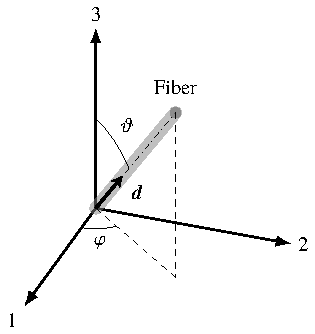
\includegraphics[scale=1]{direction_vector}
\caption{Representation of the orientation of a general fibre in the 3D space using a unit vector $\tena{d}$}\label{fig:vector5}
\end{figure}%
	
	Using the summation convention, the representative planar unit vector of a fibre is denoted as:
	\begin{equation}
	\tena{d}=d_i\tena{e}_i,\qquad i=1,2,
	\end{equation}
	where $\tena{e_i}$ is the $i$-th basis unit vector of the coordinate system, and  $d_i$ is the $i$-th component of the unit vector $\tena{d}$.

The 2nd-order planar orientation tensor ($\tenb{H}$) can be defined as~\autocite{Advani.1987}:
\begin{equation}\label{eq:one5}
H_{ij}=\int_{0}^{2\uppi}\psi(\varphi)d_id_j\text{d}\varphi,
\end{equation}
where $\psi$ is the planar probability distribution function; $d_i$ and $d_j$ are the $i$-th and $j$-th components of the unit vector $\tena{d}$, respectively. Equation~\eqref{eq:one5} can be rewritten for a discrete case consisting of $N_\text{f}$ fibres~\autocite{Ranganathan.1990}:
\begin{equation}
H_{ij}\approx\frac{1}{N_\text{f}}\sum_{k=1}^{N_\text{f}}d_i^kd_j^k.
\end{equation}
The average orientation tensor of the entire sample ($\overline{\overline{H_{ij}}}$) is obtained if $N_\text{f}$ is the total number of fibres in the sample.

	The orientation tensor is symmetric ($H_{ij}=H_{ji}$) and normalized to a unit length ($H_{ii}=1$). Therefore, only two independent components exist for a planar orientation tensor, e.g., $H_{11}$, and $H_{12}$. Namely, $H_{11}$ quantifies the proportion of alignment along the 1-axis and $H_{12}$ indicates the deviation of the coordinate axes from the principal directions of the orientation tensor~\autocite{Javanbakht.2017d}.

	The spectral form ($\tenb{H}^\prime$) of the orientation tensor ($\tenb{H}$) can be acquired~\autocite{Bertram.2015}:
\begin{equation}
\tenb{H}^\prime=\lambda_i\tena{e}_i^\prime\otimes\tena{e}_i^\prime,
\end{equation}
where $\lambda_i$ are the real eigenvalues and $\tena{e}_i^\prime$ are the normed eigenvectors forming the basis of the orthonormal coordinate system. A unique rotation $\tenb{Q}$ is used to transform the orientation tensor, by an angle equal to $\vartheta^\prime$, to the principal directions to obtain:
\begin{equation}
\mat{H}^\prime=\left[\begin{matrix}
\lambda_1& 0 \\
0 & \lambda_2\\
\end{matrix}
 \right].
\end{equation}
	An ellipse can be used to graphically represent the principal directions and values, i.e., the axes of the ellipse are directed along the principal directions and scaled according to the principal values. The major axis points to the preferred direction of the majority of the local fibres. One extreme case is to have all fibres aligned in one direction which results in a stretched ellipse with a zero minor axis, i.e., a line along the major axis. The other extreme case is a circle, which indicates no preferred orientation for the fibres~\autocite{Advani.1990,Advani.1987}.

	Analysis of the orientation of a total of $N_\text{f}$ fibres in a region can be done by partitioning the RVE into $N_\text{P}$ partitions:
\begin{equation}
N_\text{f}=\sum_{l=1}^{N_\text{P}}N_{\text{f}\,l},
\end{equation}
where $N_{\text{f}\,l}$ is the total number of fibres in the $l$-th partition. The orientation state of the $l$-th partition ($\overline{H_{ij}^l}$) is:
\begin{equation}
\overline{H_{ij}^l}=\frac{1}{N_{\text{f}\,l}}\sum_{k=1}^{N_{\text{f}\,l}}H_{ij}^{kl}.
\end{equation}
and the orientation state of the whole sample is:
\begin{equation}
\overline{\overline{H_{ij}}}=\frac{1}{N_\text{f}}\sum_{k=1}^{N_\text{f}}H_{ij}^k.
\end{equation}
From the mixing-analogy method, the clustering index $\text{[CI]}$ is defined as~\autocite{Ranganathan.1990}:
\begin{equation}
{\text{[CI]}}_{ij}=\frac{N_\text{P}-1}{N_\text{f}-1}\;\frac{[\upsigma_\text{bp}^2]_{ij}}{[\upsigma_\text{t}^2]_{ij}},
\end{equation}
where $[\upsigma_\text{bp}^2]_{ij}$ is the variance between the partitions, and $[\upsigma_\text{t}^2]_{ij}$ is the total variance. Finally, the type-1 clustering index can be expressed in terms of the orientation state as follows:
\begin{equation}
{\text{[CI]}}_{ij}=1-\dfrac{
\sum\limits_{l=1}^{N_\text{P}}\sum\limits_{k=1}^{N_{\text{f}\,l}}(H_{ij}^{kl}-\overline{H_{ij}^l})^2
}{
\sum\limits_{l=1}^{N_\text{P}}\sum\limits_{k=1}^{N_{\text{f}\,l}}(H_{ij}^{kl}-\overline{\overline{H_{ij}^l}})^2
},
\end{equation}
where the numerator indicates the sum of the variances within each partition and the denominator is the variance of the whole RVE.

\red
\section{Micro-mechanical Model for Discontinuous Fibres}
	The extension of the Eshelby model~\autocite{Eshelby.1957,Eshelby.1961} to heat transfer problems is the Hatta-Taya model~\autocite{Hatta.1985,Taya.1989}. In either model, the equivalent inclusion technique is adopted by introducing a transformation tensor that creates a homogeneous medium from the composite with heterogeneities. Thereof, an eigen-quantity~\autocite{Mura.1987} is related to its constraint counterpart. Such an approach is common in Duhamel-Neumann type equations~\autocite{Javanbakht.2019b,Ghosh.2011}. In its classic derivation, such a relation is established by the Eshelby tensor, which depends on the geometry of the inclusions. Herein, ellipsoidal inclusions (Eshelby's template for inclusions) were adjusted to properly represent short fibres. The three semi-diameters $a_1$, $a_2$, and $a_3$ of spheroids are named along the axis of the coordinate system $\left\{\tena{e}_i\right\}\equiv\left\{\tena{e}_i\right\}_{i=1}^3$. Short fibres are considered as oblate spheroids ($a_1=a_2\ll a_3$) in this model, and the components of the Eshelby tensor are explicitly calculated as \begin{subequations}
		\begin{alignat}{2}
			S_{11}=S_{22}&=\frac{\beta}{2\sqrt{(\beta^2-1)^3}}\left(\beta\sqrt{\beta^2-1}-\cosh^\inv\beta \right),\\
			S_{33}&=1-2S_{22},
		\end{alignat}
		\end{subequations}
	where $\beta\equidef\sfrac{a_3}{a_2}$ is the aspect ratio of the fibres.

	In the formulation of Hatta-Taya model for 2D (on the 1-3 plane), the angle $\alpha$ denotes the range of fibre distribution and $\theta$ is the angle of the fibres, i.e., $0\le \alpha\le\sfrac{\pi}{2}$ and $-\alpha\le \alpha\le\alpha$. The $\rho\equiv\rho(\theta)$ function defines the number of fibres per unit area of the $\mathbb{S}^2$ unit sphere in 3D, which reduces to $\mathbb{S}^1$ unit circle for 2D. In order to model the aligned fibre case, $\alpha\rightarrow 0$ and $\rho\equimust\delta(\theta)$ in which $\delta(\theta)$ is the Kronecker delta generalised function. Furthermore, assuming isotropic materials for both fibre ($\tenb{k}_\text{f}\equiv k_\text{f}\unitb$) and matrix ($\tenb{k}_\text{m}\equiv k_\text{m}\unitb$) phases, the auxiliary tensor
	\begin{equation}
		\tenb{A}\equidef (k_\text{f}-k_\text{m})\unitb\scp\tenb{S}+k_\text{m}\unitb,
	\end{equation}
	is used along with the Eshelby tensor to calculate
	\begin{subequations}
	\begin{alignat}{3}
		Q_1^*        &\equidef (k_\text{m}-k_\text{f})A_{11}^\inv,\\
		Q_3^*        &\equidef (k_\text{m}-k_\text{f})A_{33}^\inv,\\
		Q_1^\text{C} &\equidef (k_\text{m}-k_\text{f})S_{11}A_{11}^\inv,\\
		Q_3^\text{C} &\equidef (k_\text{m}-k_\text{f})S_{33}A_{11}^\inv.
	\end{alignat}
	\end{subequations}
	Finally, the axial (along the 3-axis) and transverse (along the 1-axis) effective properties are calculated by
	\begin{subequations}
	\begin{alignat}{2}
		k_\text{axial} &= k_\text{m}\left( 1 - \frac{\zeta_{\text{f}}Q_3^*}{\zeta_{\text{f}}Q_3^\text{C}}   \right),\\
		k_\text{trans} &= k_\text{m}\left( 1 - \frac{\zeta_{\text{f}}Q_1^*}{1+\zeta_{\text{f}}Q_1^\text{C}}   \right).
	\end{alignat}
	\end{subequations}
	


\bl

\section{Methodology}
	In the current study, the finite element method~\autocite{Ochsner.2013,Oechsner.2016,Ochsner.2018,Javanbakht.2017c} was used to estimate the effective thermal conductivity of randomly oriented short fibres with clustering. A Python script is used to create the parametric FE model, run the job submissions, and post-process the resulting data. This procedure was embedded in the MSC.Marc (version 2017.0) commercial finite element package, and thus has the advantage of automating the whole process~\autocite{Javanbakht.2016,Javanbakht.2016b,Javanbakht.2017}.

\begin{figure}
\centering
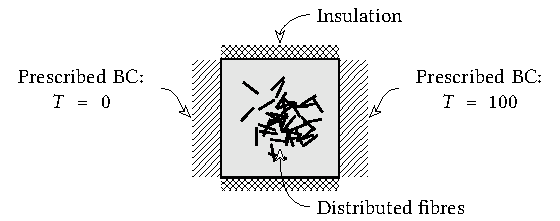
\includegraphics[scale=1]{HC2_RVE_sample.pdf}
\caption{Schematic illustration of the prototype RVE}\label{fig:RVE5}
\end{figure}%

	Dimensionless values were used throughout the investigation, and thus normalized results will be discussed. All the FE models where generated based on a 2D prototype RVE ($10\times10$), which consists of 4-node bilinear isoparametric planar heat transfer elements (type 39) for the matrix phase and straight 2-node link elements (type 36) for fibres, see Fig.~\ref{fig:RVE5}. The contrast of the properties is chosen to be 600, i.e., thermal conductivities of $1$, and $600$ for the matrix and fibres, respectively. An aspect ratio of $40$ was acquired for the fibres, i.e., a fibre length of $5$ and a diameter of $0.125$, to stay within the range of $20$\thinspace--\thinspace$60$ aspect ratios of the short fibres~\autocite{Kalpakjian.2010}.
	
	Considering the effectiveness of boundary conditions~\autocite{Javanbakht.2017b}, the recommended prescribed temperature boundary condition is used~\autocite{Islam.1999}. A temperature gradient of 100 is imposed to set up a steady-state flux across the RVE, see Fig.~\ref{fig:RVE5}. After steady state heat transfer analyses, the reaction flux is collected from the right-hand boundary nodes and summed up to obtain the total heat flux~\autocite{Rakovsky.2014}. Then, the effective thermal conductivity of the RVE is calculated using Fourier's law~\autocite{Fiedler.2009}:
	\begin{equation}
	k_{\text{eff}}=\frac{\dot{Q}}{A_0}\cdot\frac{\mupDelta z}{\mupDelta T},
	\end{equation}%
	where $k_{\text{eff}}$ is the effective thermal conductivity of the RVE, $\dot{Q}$ is the sum of the generated reaction fluxes on the right-hand boundary, $A_0$ is the assumed cross-sectional area (with a thickness of unit length) perpendicular to direction of the flux, $\mupDelta z$ is the distance between the edges of the sample, and $\mupDelta T$ is the prescribed temperature gradient.

Note that a mesh sensitivity analysis was carried out to remove the mesh dependency of the values of effective thermal conductivity. It was carried out over a range of uniform mesh densities ($\gamma$) from 1 to 35~\autocite{Javanbakht.2018}:
\begin{equation}
\gamma=\frac{1}{\ell_\text{mesh}},
\end{equation}
where $\ell_\text{mesh}$ was the edge length of the used square elements. The results showed that the mesh sensitivity was diminished for $\gamma$ over 20 and thus, it was selected as the prototype mesh density for all the simulations.

	The following assumptions are made for creating all the models:
	\begin{itemize}
		\item The thermal conductivity is independent of the temperature.
		\item The transverse conductivity of the fibres is negligible.
		\item A perfect bonding exists between the fibres and matrix, i.e., the thermal barrier resistance is disregarded.
		\item In generating the distributions, overlapping of the fibres is ignored since no explicit cross-section is considered for fibre elements.
	\end{itemize}
	The RVE is divided into four equal partitions which incorporated fibres with equal volume fractions. The locations of the fibres are selected randomly and their orientation followed a von Mises distribution~\autocite{Mardia.1975}. The mean value of the distribution was kept to $\mu=0$ so the fibres are oriented along the direction of the heat flow, see Fig.~\ref{fig:case5}. However, in order to investigate the effect of orientation distribution, the concentration parameter ($\kappa$) was modified from 0 to 50 in the two rightmost partitions to consider the random and highly oriented cases, respectively. 
\begin{figure}[!h]
\centering
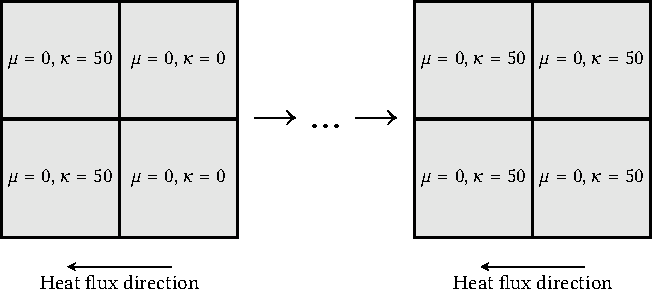
\includegraphics[scale=1]{hc2_RVE}
\caption{Two extreme cases of fibre distribution in the RVE---the fibre volume fraction is kept the same in each partition}\label{fig:case5}
\end{figure}%

\red
	\paragraph{Model validation} In Chapter~\ref{chap:p4}, the results in~\autocite{Fu.2003,Choy.1994} were used to validate the computational model. It was shown that the Hatta-Taya model~\autocite{Hatta.1986,Taya.1989} provided a good agreement with the results. Therefore, the Hatta-Taya model was used to benchmark the FE prototype. The 2D prototype is analysed with the same aforementioned parameters. However since the von Mises distribution was used for planar distribution of fibres, an extreme value for concentration parameter ($\kappa=800$) was chosen to simulate the aligned fibre distribution. 
		
	The response of the FE prototype for aligned short fibres along with the values of the Hatta-Taya model are depicted in Fig.~\ref{fig:hc2_val}. It can be seen that the current model shows a good correlation with the Hatta-Taya model for a wide range of fibre volume fractions. At higher fractions of fibres, the computational model underestimates the effective thermal conductivity.
\begin{figure}[!h]{}
  \centering
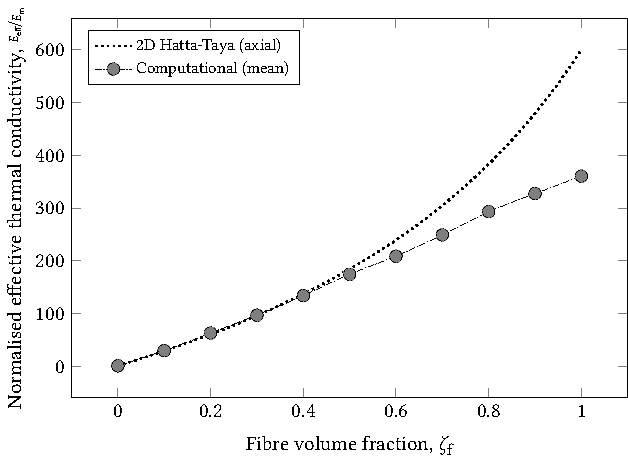
\includegraphics[scale=0.9]{hc2_validation}
  \caption{Validation of the model with the results provided in~\autocite{Fu.2003,Choy.1994}}
  \label{fig:hc2_val}
\end{figure}	
 	In Table~\ref{table:hc2_validation}, the percentage relative error of the computational model with respect to the axial thermal conductivity of the Hatta-Taya model is presented. The computational results show a very good agreement with the benchmark analytical model up to 50\% fibre volume fraction; the percentage relative error remains below 5\%. For higher fibre volume fractions, the model underestimates the thermal conductivity. The maximum error of 40\% is obtained for 100\% fibre volume. Nevertheless, the FE prototype in the current study is used to simulate a low fibre volume fraction of 10\%, and thus can be used confidently.
		
\begin{table}[!h]
\centering
\caption{Effective thermal conductivity results of the computational model against results of the Hatta-Taya micromechanical model.}\label{table:hc2_validation}
\small
\begin{tabular}{*{3}{P{0.07\textwidth}}P{0.1\textwidth}}
\toprule
  $\zeta_{\text{f}}$ \bfs{(\%)}
& {$\frac{k_\text{axial}}{k_\text{m}}$} 
& {$\frac{k_\text{comp}}{k_\text{m}}$} 
& $e_\text{comp}$ \bfs{(\%)}
\\
\toprule
0.10&28.98 & 29.63&-2.22\\
0.20&60.49& 63.16&-4.42\\
0.30&96.22& 96.96&-0.76\\
0.40&137.10& 133.94& 2.31\\
0.50&184.33& 174.55& 5.30\\
0.60&239.49& 208.86&12.79\\
0.70&304.79& 249.09&18.27\\
0.80&383.30& 293.17&23.51\\
0.90&479.46& 327.49&31.70\\
1   &600& 360.58&39.90\\
 \bottomrule
\end{tabular}
\end{table}	

\bl
Finally, a statistical analysis was carried out for each sample by dividing the RVE into four equal partitions. The orientation tensors of the fibres were obtained along with their principal values and directions in each partition and the whole RVE. Finally, the clustering index was calculated for the RVE and correlated with the values of the effective thermal conductivity.  

%TODO would it help to descretize the fibre elements as well?
% ──────────────────────────────────────────────────────────────────────────────────────────────────
\section{Results and Discussion}
	The main focus of the current study was on randomly-oriented fibres, and thus the selection of a pseudo-random algorithm will highly affect the result of the study. Therefore, a von Mises distribution was considered for the orientations to obtain a more controllable approach. In order to challenge the validity of the clustering index, the two rightmost partitions underwent a transition from a random orientation state ($\kappa=0$) to a more concentrated state ($\kappa=50$). This parameter change was applied to fibre volume fractions above the non-dilute limit, i.e., volume fractions from 10\,--\,40\%. The effective thermal conductivity was also calculated in each case and normalized with respect to the thermal conductivity of the matrix.

	Increasing the fibre volume fraction increased the effective thermal conductivity of the composite, see Fig.~\ref{fig:cond5}. Increasing the concentration parameter of the von Mises distribution located more fibres about the flow direction, and thus the thermal conductivity increases. Although the orientation of fibres highly affected the thermal conductivity, this effect seemed to diminish in concentration parameters of more than $\kappa=20$. Furthermore, the effective thermal conductivities showed a lower standard deviation at higher concentration parameters, which is highly noted in lower fibre volume fractions. Namely, by increasing the concentration parameter, more consistent thermal conductivity values were obtained especially for low fibre volume fractions; the latter behaviour can be attributed to the decrease of randomness at low volume fractions.

\begin{figure}[!h]
  \centering
	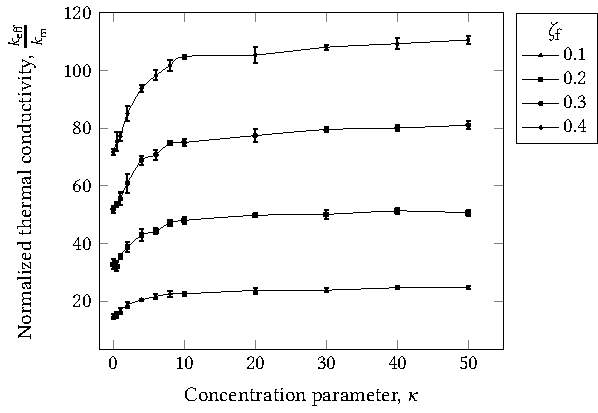
\includegraphics[scale=0.9]{hc2_conduc}
  \caption{Normalized effective thermal conductivity for different concentration parameters and volume fractions}
  \label{fig:cond5}
\end{figure}%

Detection of clustering was investigated using the clustering index obtained from the mixing analogy~\autocite{Ranganathan.1990}. In the case of clustering, it was assumed that a preferred orientation existed along which fibres locally co-orient themselves. The clustering index varies between 0 and 1 where the former indicates a cluster-free state and the latter indicates a clustered state.

The $H_{11}$ component indicates the strength of fibre alignment along the direction of the heat flux whereas the $H_{12}$ component quantifies the dissimilarity in the principal directions of orientation in the partitions of the RVE. The clustering index for component 11 and 12 of the orientation tensor is illustrated in Figs.~\ref{fig:ci11} and \ref{fig:ci12}, respectively. A clustered state was detected for the $H_{11}$ component at the low values of the concentration parameter whereas no clustering was found for the $H_{12}$ component. In addition, a higher standard deviation was observed for the low concentration parameter region, i.e., $\kappa$ less than 20. 

	\begin{figure}[!h]
	\centering
	\subfloat[Clustering index 11 for different concentrations and volume fractions\label{fig:ci11}]{	\includegraphics[scale=0.8]{hc2_c11}}\hfill
	\subfloat[Clustering index 12 for different concentrations and volume fractions\label{fig:ci12}]{	\includegraphics[scale=0.8]{hc2_c12}}
	\caption{Clustering indices of the analysis}\label{figure:hc2_clus}
	\end{figure}%

	Although modest values was generally obtained for the clustering index $[CI]_{11}$, clustering (if any existed) seemed to fade at higher concentration parameters. By increasing the concentration parameter, the clustering state for $H_{11}$ weakened and became negligible for concentration parameters more than 30. Note that no interesting change was observed for the other index, i.e., it indicated a more or less similar principal direction in all cases, see Fig.~\ref{fig:theta}. Namely, no strong orientation tendency was detected. More importantly, no remarkable change was detected by increasing the volume fraction. Thus, one could argue that the orientation tensor is not affected by the fibre volume fraction in the case of uniform distribution of fibre volume. The maximum principal value of the orientation tensor approached to unity by increasing the concentration parameter, see Fig.~\ref{fig:lambdamax}. Namely, orientation of the fibres can be enforced along the flow direction by increasing the greatest eigenvalue---provided that the principal direction remains the same.

\begin{figure}[!h]
	\centering
	\subfloat[Rotation to principal direction with respect to the 1-direction\label{fig:theta}]{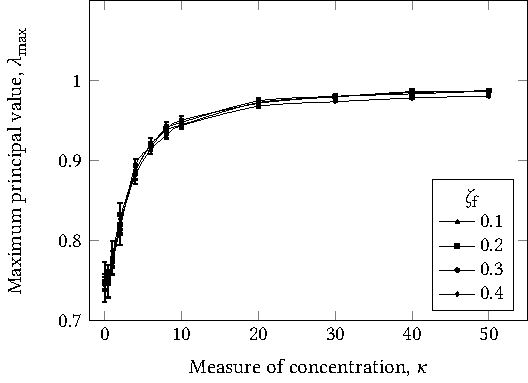
\includegraphics[scale=0.8]{hc2_lambda}}\hfill
	\subfloat[Maximum principal value of the orientation tensor for different concentrations and volume fractions\label{fig:lambdamax}]{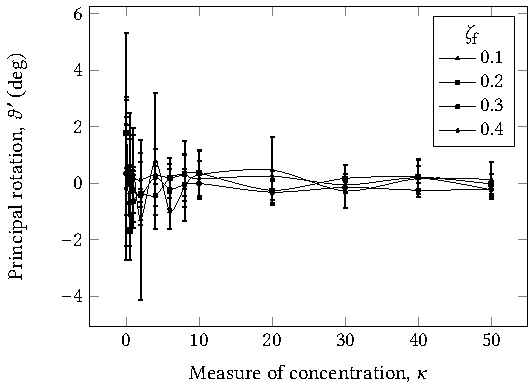
\includegraphics[scale=0.8]{hc2_theta}}
	\caption{Results of spectral analysis}\label{fig:hc2_spectral}
\end{figure}


\section{Conclusion}
\red
	The current study attempted to relate the effect of fibre clustering and effective properties of an RVE. It was observed that by increasing the concentration parameter, the strength of clustering decreases while the orientation clustering remains unaltered.\bl~It can be concluded that increasing the fibre volume fraction increases the effective thermal conductivity of the composite. This is highly effected by the orientation state of the fibres, i.e., a clustered fibre distribution may inhibit the heat flux. Moreover, orienting the fibres along the heat flow facilitates heat transfer---provided that clustering is minimum. This is true specially when the principal direction of the fibres remains along the heat flow and the clustering index does not change along this direction. Finally, by increasing the maximum principal value of the orientation tensor, alignment of the fibres can be further enforced along the flow direction which results in an efficient use of fibres for improving thermal conductivity. This approach can be used to characterize the composite and determine its degree of efficiency in terms of fibre engagement both in thermal in mechanical aspects of a composite.
